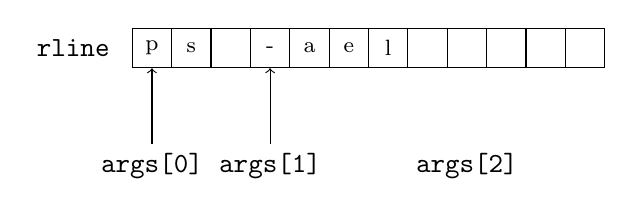
\begin{tikzpicture}
\tikzstyle{box} = [minimum width=0.5cm, minimum height=0.5cm, draw, font=\footnotesize];

\foreach \x/\y in {1/p,2/s,3/,4/-,5/a,6/e,7/l,8/,9/,10/,11/,12/}
	\node[box] (n-\x) at (\x*0.5,0) {\y};

\node at (-0.5,0) {\texttt{rline}};
\node (t-0) at (0.5,-1.5) {\verb"args[0]"};
\draw[->] (t-0) edge (n-1);
\node (t-1) at (2,-1.5) {\verb"args[1]"};
\draw[->] (t-1) edge (n-4);
\node at (4.5,-1.5) {\verb"args[2]"};
\end{tikzpicture}